\documentclass{article}
\usepackage{imakeidx}
\usepackage{graphicx}
\usepackage{wrapfig}
\usepackage{mathtools}
\graphicspath{{images/}}
\usepackage{geometry}
\usepackage{circuitikz}
\geometry{a4paper,
total={170mm, 257mm},
left = 30mm,
right = 30mm,
bottom = 30mm,
top = 30mm
}

\usepackage{multicol}
\title{Computer Systems and Architecture \linebreak Revision Notes}
\author{James Brown}
\makeindex
\begin{document}
	\pagenumbering{gobble}
	\maketitle
	\newpage
	\tableofcontents
	\newpage
	\pagenumbering{arabic}
	
	\section{Introduction}
	These are notes I have written in preparation of the 2017 Computer Systems and Architecture exam. This year the module was run by Iain Styles (I.B.Styles@cs.bham.ac.uk). This is the module did not cover networks and they are not examinable - as such I will not be writing about them here.
	
	\section{Fundamentals of Computer Organisation}
	Computer programs consist of \textbf{instructions}\index{instructions} and \textbf{data}\index{data} which are identical in appearance, but they are logically distinct. Programs have a ordered set of instructions which are executed sequentially, unless it's otherwise stated. Programs also have data which is there to be manipulated by the instructions which are run. In the computers memory these will both have the same physical representation, but are not the same as each other. Because of this, when storing instructions and data they must be kept logically separate. That is to say they must be stored in different regions of memory, and not interspersed with each other for example.
	
	\par 
	We may want to describe the computers architecture at a variety of levels of abstraction:
	\begin{itemize}
		\item \textbf{Level 5}: High Level Languages\index{high level language}. These are largely independent of the physical machine, occasionally regarded as part of the architecture.
		\item \textbf{Level 4}: Assembly Language\index{assembly language}. Programming in terms of the machine's basic operations.
		\item \textbf{Level 3}: Operating System\index{operating system}. Common services and management functions.
		\item \textbf{Level 2}: Instruction Set\index{instruction set}. The basic operations that the machine can execute.
		\item \textbf{Level 1}: Microarchitecture\index{microarchitecture}. The distinct functional units that are required to implement the instruction set, and their organisation.
		\item \textbf{Level 0}: Digital Logic\index{digital logic}. The implementation of the functional units in terms of basic logic operations.
		\item \textbf{Level -1}: Physical Device. The implementation of the logic using basic electronic components such as transistors\index{transistor}, and the physical substrate on which these are constructed.
	\end{itemize}
	
	\subsection{The von Neumann Architecture and Executing Programs}
	\subsubsection{von Neumann Architecture}
	\begin{figure}[h]
		\centering
		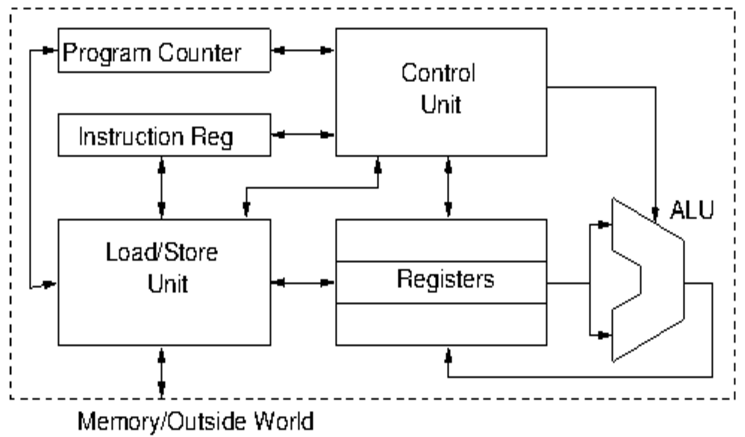
\includegraphics[width=0.6\textwidth]{von_neumann}
		\caption{The von Neumann Architecture}
		\label{fig:von neumann}
	\end{figure}
	
	Many modern computers are built on the (or use slightly modified) von Neumann\index{von Neumann architecture} architectures and can be considered it's heart. 
	
	\par	
	We consider the main memory\index{main memory} as being logically - but not necessarily physically - separate from the CPU. The main memory holds all of the instructions and data that make up a program(s). As stated earlier, instructions and data are stored in distinct locations within the main memory so that they are easily distinguished. Within main memory, instructions are stored sequentially so that you can determine the flow of the program implicitly from their order. Lastly, main memory is also a volatile\index{volatile} storage method, meaning that all data is lost once the power is cut.
	
	\par 
	The \textbf{Load/Store unit}\index{load/store unit} is used as the interface between the CPU and the outside world. It issues and receives requests to transfer instructions and data between the CPU and the memory via the bus.
	
	\par
	The \textbf{registers}\index{registers} are small amounts of local, fast access storage the hold data that is currently in use. Data is passed to the registers by the load/store unit. Each register can hold one 'word' of data. The main registers are used purely to hold data - instructions are dealt with separately.
	
	\par 
	The \textbf{instruction register}\index{instruction register} hold the current instruction that is being executed so that it can be used by the control unit\index{control unit} to configure the ALU\index{ALU}. Only one instruction is active at any one time, unless the design features special techniques for performance improvements that rely on multiple instructions being executed simultaneously.
	
	\par 
	The \textbf{ALU (arithmetic and logic unit)}\index{ALU}\index{arithmetic and logic unit} is the 'engine' of the computer. It performs all the computations and comparisons. It also reads data from registers and writes the results of calculations back into the registers.
	
	\par 
	The \textbf{program counter}\index{program counter} is a special register that contains the memory location (address) of the next instruction which shall be executed - a bookmark in essence. In the normal execution of a program, the program counter is incremented after each instruction to point to the next memory location. Some instructions may change the value of the program counter in order to change the order of execution.
	
	\par 
	Additionally, we may want to add some other components just outside of the CPU which can be just as important. Due to the fact the main memory is remote from the CPU, access times can be slow. We may use an intermediate layer of memory known as \textbf{cache}\index{cache} that is smaller but much faster to access. This would be used to hold portions of programs that are likely to be used again shortly. We may also want to use stable, \textbf{long-term memories}\index{long-term memory} such as disks or DVDs. Typically these all will require the use of an \textbf{Input-Output (IO) controller}\index{IO controller} which handles peripheral devices such as disk drives, mice and keyboards. It may do this through an extension of the memory addressing protocol or via an interrupt based protocol. Memory, peripherals and the CPU all communicate with each other via the \textbf{bus}\index{bus} which carries data around and allows, for example, data to be transferred from disk into main memory. This bus consists of a set of physical wires plus a protocol (there are many available, such as PCI, ISA, IDE, SCSI) that is implemented by the \textbf{bus controller}\index{bus controller}. The bus controller determines which subsystems can communicate. It should be noted that only one piece of data can be on the bus at any time.
	
	\subsubsection{The Clock Cycle}
	The vast, vast majority of computer systems are \textit{synchronous} - meaning their activities are synchronised by an external clock signal in the form of a \textbf{square-wave electric pulse}. This speed is frequently quoted as a measure of CPU performance but to say it is analogous to performance would be slightly false. There are many other factors and different architectures cannot be compared on the basis of their clock rate alone. The time between two different pulses is related to the frequency of the CPU by $t = 1 / f$ and is called a cycle time.
	
	\par 
	For the most part computer systems must be synchronus as variability in manufacturing means that it's not possible to know exactly how long it will take for a particular operation to complete. The clock cycle is chosen to be slightly longer than the longest delay in the system which ensure the machine is in a well defined state when the next set of operations start which is triggered by the \textbf{rising edge} of the clock pulse.
	
	\subsubsection{Executing Programs}	
	Computer programs, in their most basic form, are just sequential series' of instructions. In von Neumann architecture, the execution of these instructions is governed by the \textbf{instruction execution cycle}\index{instruction execution cycle}. The instruction execution cycle is triggered by the clock cycle, but has several stages within it which are triggered by successive clock pulses. One complete instruction cycle usually takes several clock cycles to execute - exact numbers depend on the type of instruction and the details of the particular machine. Fetch data from memory for example may take several clock cycles to execute, and it may take several cycles before the data is safely loaded into a register. Others may complete in a single clock cycle such as the addition of the contents of two values stored in registers.
	
	\par 
	Most architectures follow the same basic set of stages in the \textbf{Fetch-Decode-Execute Cycle}\index{fetch-decode-execute cycle}. In can roughly be broken down into 8 steps in an idealised version:
	
	\textbf{Fetch:}
	\begin{enumerate}
		\item Inspect the program counter to find the address of the next instruction
		\item Load the next instruction from memory into the instruction register
		\item Update the program counter to point at the next instruction
	\end{enumerate}
	
	\textbf{Decode:}
	\begin{enumerate}
		\setcounter{enumi}{3}
		\item Determine the type of instruction fetched
		\item If the instruction requires data from memory, determine its address (usually embedded in the instruction
	\end{enumerate}
	
	\textbf{Execute:}
	\begin{enumerate}
		\setcounter{enumi}{5}
		\item Fetch and required data from memory into one of the CPU registers
		\item Execute the instruction
		\item Return to step 1 for the next instruction
	\end{enumerate}
	
	Starting a program doesn't fit neatly into this simple model and before we enter the cycle we also need to take a few actions to make sure that things are ready. Firstly, we need to load the program from disk into main memory\index{main memory}. The instructions and data needed by the program will each occupy a block of memory, which is allocated by the operating system, and the memory address of the first instruction is called the \textbf{entry point}\index{entry point}. When first started, the entry point is loaded into the program counter which then becomes the starting point of the cycle.
	
	\par 
	\textbf{Fetch}. Once we have a valid instruction location in the program counter (PC), we can begin the cycle. An important note is that at this point in time all we have is the memory address - not the actual instruction - we still need to actual fetch it, hence the title. At the start of the next clock cycle, the CPU issues a request via the load/store unit to the memory by sending the memory address and a request to read from the memory via the bus. Later in time, the instruction will be received from memory by the load/store unit and then stored in the instruction register (IR). Depending on the relative speed of the clock cycle and the memory, it could take several cycles before the instruction is ready in the IR. Once the request  has been made, the value of the PC is changed to point to the next instruction - which usually just involves simply incrementing the PC. This may however be modified by some instructions such as \texttt{branch} or \texttt{jump}.
	
	\par 
	\textbf{Decode}. Now we have the instruction in the IR, we can begin to act upon it in the CPU. The type of instruction is determined by the control unit. This is necessary in order to determine if any further actions needs to be taken in order to execute this instruction.
	
	\par 
	\textbf{Execute}. After finding the type of instruction, any data needed is fetched from the memory. For a lot of CPUs, most instructions can only actually access registers and there are dedicated instructions for accessing main memory. Once the data is in the registers, it can be operated upon. As mentioned earlier, some instructions change the flow of the program and are therefore allowed to change the PC as necessary (when doing this it is often required for the previous value of the PC to be stored so that execution can resume once the branch has completed).
	
	\subsection{Harvard Architecture}
	In the von Neumann architecture, instructions and data are accessed via the same physical and logical pathway (the load/store unit) and there is not formal separation between data and instructions at this level. In this case, the two types of information are stored in the same physical memory but are separated by their locations within the memory. This separation is common practice in all computers as it allows for dynamic repartitioning of the memory according to the needs of the program. The problem is due to the fact that by having a shared interface, instructions and data cannot be accessed simultaneously. This is known as the \textbf{von Neumann bottleneck}\index{von Neumann bottleneck} and it restricts CPU performance to the rate at which is can be supplied with data.
	
	\par 
	A potential solution is to provide separate memories for small amounts of instructions and data that are likely to be used soon - separate instruction and data caches. It is also common to provide separate interfaces to instruction and data memory which is known as the \textbf{Harvard architecture}\index{harvard architecture}. In a pure implementation of the Harvard model, instructions and data are stored in physically separate memory but this is not flexible enough for general purpose computational devices that has a single unified memory space. The \textbf{modified Harvard architecture} has a single unified memory space (that is partitioned for instructions and data) but with separate buses for instructions and data. In most modern machines, this is the approach that is taken.
	
	\subsection{Case Studies}
	\subsubsection{MIPS}
	The MIPS processor is the canonical example of a modified Harvard architecture and is very similar to the von Neumann model shown earlier. It features an instruction register, a program counter, an ALU etc, but has separate pathways for accessing instructions and for accessing data. In the diagram they are shown as physically separate, but in reality they are part of a physically unified memory.
	
	\begin{figure}[h]
		\centering
		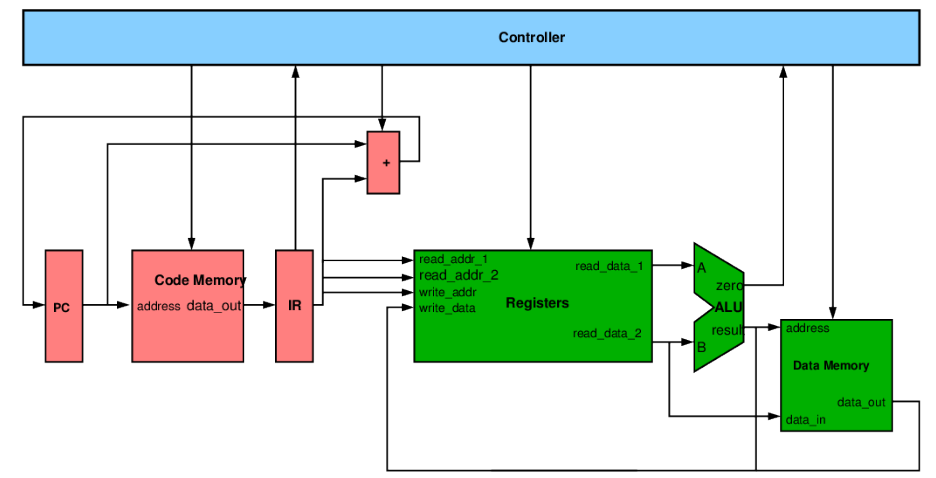
\includegraphics[width=\textwidth]{mips_architecture}
		\caption{The MIPS processor}
		\label{fig:mips processor}
	\end{figure}
	
	\subsubsection{Intel x86}
	Modern versions of x86 are much more complex when compared to the relatively simple MIPS Harvard based architecture. This is partly down to the fact that MIPS has around 60 simple instructions whereas the latest Intel Core machines have hundreds of instructions - many of which are not simple. The benefit of these additional instructions for the x86 architecture is a significant increase in performance and it can also make it easier for the programmer/compiler writer. This all comes at the cost of a much more complex design - MIPS R4000 contains 1.2 million transistors. A quad-core i7 processor on the other hand has 731 million transistors on a die that is not much larger than that in a MIPS machine. One of the main features of modern Core architecture is that it is highly superscalar and can execute multiple instructions simultaneously. Due to this, the CPU requires several ALUs, several instruction decoders, instruction queues and multiple levels of caching. If you can see through all the complexity, you can see that the Core 2 is essentially a modified Harvard architecture.
	
	\section{Instruction Sets and Assembly Language}
	One of the major defining features between different computers is the choice of \textbf{instruction set}\index{instruction set}. Modern computers are \textit{Turing-complete}\index{turing complete} - meaning they can perform any computation that can be performed - so in some sense the set of instructions doesn't matter as long as they implement a Turing-complete system. In practice, the choice of instructions can greatly affect the programmers task - especially for very low level programming.
	
	\par 
	Each type of CPU has a different instruction set which are effectively incompatible with each other. Some machines have instructions that other do not and some may have identical instructions with different binary representations. Due to this, low-level code is extremely machine dependent and written by hand only when totally necessary. Due to the widespread use of von Neumann and Harvard architectures different instruction sets tend to have a general similarity.
	
	\subsection{Types of Instruction Set}
	Instruction sets are frequently classified as \textbf{complex} (Complex Instruction Set Computer\index{complex instruction set computer} - \textbf{CISC}, Intel designs for example) or \textbf{reduced} (Reduced Instruction Set Computer\index{reduced instruction set computer}- \textbf{RISC}, for example ARM and MIPS). 
	
	\par	
	CISC computers generally have a very extensive range of instructions (this tends to be in the area of several hundered). These can range from simple instructions like addition and subtraction to more complex operations that are often common combinations of simpler instructions to provide specific support for high-level functions. CISC instruction sets have the advantage of possibly making the translation of high-level software into machine language somewhat easier. Microcoding\index{microcoding} of the complex instructions can also provide a performance benefit over their implementation in software. One drawback is the added complexity of the hardware which may make debugging and optimisation very difficult. The biggest example of CISC processors is the Intel x86 family which even includes instructions such as \texttt{AESDEC} to perform AES decryption.
	
	\par 
	RISC machines are the opposite of CISC machines - the number of instructions is minimised and each instruction is highly optimised with the ability to make use of performance-enhancing measures such as pipelining and speculatice execution. A popular RISC machine is the MIPS architecture which was very popular in the 1990s but continues to be widely used in embedded systems because of its low power and heat generation. The basic instruction set has around 60 instructions (some MIPS variants did have more), and these are \textbf{superpipelined}. Key points on the MIPS architecture:
	\begin{itemize}
		\item 32-bit architecture (instructions, memory addresses and words of data are 32 bits long)
		\item 32 data registers, \$0 ... \$31. \$0 is a special register and reserved for the value zero. Other registers are reserved for other special purposes by convention only.
		\item Most instructions can only interact with registers - there are special instructions for transferring data to/from memory. Due to this, some stages of the instruction cycle can be omitted.
		\item Byte-addressed, meaning that an increment of 1 in the program counter points to the next byte, not the next word. This makes the normal PC increment 4, not 1.
	\end{itemize}
	
	\subsection{Types of MIPS Instructions}
	Instructions of the MIPS processor can be divided into eight rough categories:
	
	\par 
	\textbf{Load/Store Instructions} which fetch/store items from/to memory. Several variants which work on whole(32-bits) or part-words(half-words or bytes).
	
	\par 
	\textbf{Arithmetic Instructions} which are used to add/subtract etc. two variables being held in the registers, and also to perform comparisons.
	
	\par 
	\textbf{Immediate Arithmetic Instructions} which are similar to regular arithmetic instructions but used to specifically add/subtract a constant and a variable in a register.
	
	\par 
	\textbf{Shift Instructions} which are used to perform bit rotations - commonly used in cryptographic protocols
	
	\par 
	\textbf{Multiply/Divide Instructions} which perform multiplication or division on two variables being held in the registers.
	
	\par 
	\textbf{Jump and Branch Instructions} which are used to change the normal sequential flow of program instructions. For example, to call subroutines, take branches in the code (at conditionals) and implement loops.
	
	\par 
	\textbf{Coprocessor Instructions} which are used to send data and pass control to an external coprocessor which might, for example, be a graphics controller or external floating-point processor.
	
	\par 
	\textbf{Special Instructions} which do no fall into any of the above categories. In this course, we don't consider these at all.
	
	\par 
	To begin, we'll consider the most common instructions and how they relate to high-level code. Consider the simple code \texttt{a = a + b;}. In the MIPS instruction set, we have an instruction called \texttt{add} which takes three \textbf{operands} - analagous to arguments of functions in higher-level languages. The three operands are the \textbf{destination} of the result, and the two \textbf{sources} of the inputs. Arithmetic instructions can only access the registers so the operands must specify which registers are to be used. Therefore, we may translate our simple example into \texttt{add \$8, \$8, \$9}. This adds the contents of the register 8 to the contents of the register 9, and stores the result into register 8. The order of the operands is important here, the destination comes first!
	
	\par
	This code assumes the values of the variables \texttt{a} and \texttt{b} are already in the registers. We will need instructions to load data from memory into the registers and to store the result from registers into memory. An instruction to load a word of data from the memory will need operands which specify which register the data should be loaded into and where in the memory it will come from. For the moment, we will denote memory addresses using C-like notation such as \texttt{\&a}. The instruction \texttt{lw \$8, \&a} loads the contents of a word of data at memory address \texttt{\&a} and puts it in register \texttt{\$8}. It follows that we also have a function \texttt{sw \$8, \&a} which takes the contents of a register and stores that word at the specified memory address. We can modify our program to load \texttt{a} and \texttt{b} from memory and to then store \texttt{a} in memory after performing the addition:
	
	\begin{verbatim}
	lw $8, &a;
	lw $9, &b;
	add $8, $8, $9;
	sw $8, &a;
	\end{verbatim}
	
	This alone does not make up a full MIPS program. We must add various assembler directives and also encapsulate this code into a main function in order to be able to run it.	
		
	\subsection{MIPS Register Conventions}
	
	\begin{figure}[h]
		\centering
		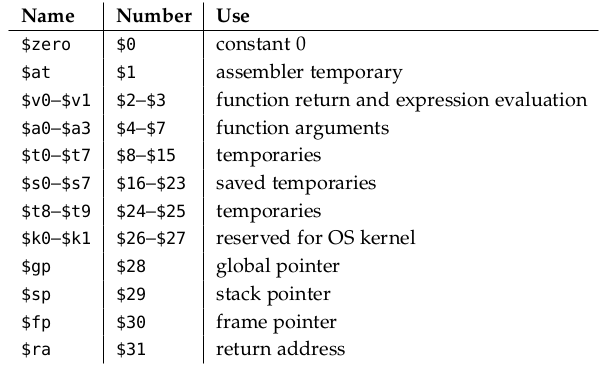
\includegraphics[width=0.7\textwidth]{mips_register_conventions}
		\caption{The conventions of use for all registers in the MIPS architecture}
		\label{fig:mips register conventions}
	\end{figure}
	
	While all registers apart from \texttt{\$0} is freely accessible by the programmer there is still a convention for their use. Their conventions are shown in Figure \ref{fig:mips register conventions}. Important registers are \texttt{\$8} through \texttt{\$15} which are for 'temporaries' and we can use them to store intermediate values. The assembler also supports the use of the register names rather than numbers, so those will be used from now on making to code a little more readable.
	
	
	
	\subsection{Machine Code}
	All MIPS instructions are 32 bits long, with the 32 bits divided into sections. The precise division of bits depends on the type of instruction. If we consider the simple arithmetic operations we have used in our examples, the machine level representation must include information about what operation is to be performed and which registers should be used. The precise format for this type of instruction (called a \textbf{register operation}\index{register operation} is shown below.
	
	\begin{figure}[ht]
		\centering
		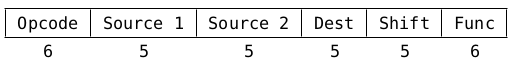
\includegraphics[width=0.7\textwidth]{rtype_instruction}
		\caption{MIPS instruction format for register operations}
		\label{fig:mips register operations}
	\end{figure}
	
	The \textbf{opcode} field of 6 bits describes which type of instruction is being described (not the specific instruction). This is important as it determines how the rest of the instruction is going to be interpreted. The remaining bits are used to encode the two \textbf{source} registers and the \textbf{destination} register as 5 bit numbers; a \textbf{shift} field which is used by certain bit-shifting operations and denotes how far the shift should be; and finally the \textbf{func} fiedl which encodes exactly which instruction is desired. All register type instructions follow the same flow of information so having single opcode for all such instructions simplifies things significantly. We can then use the func code to configure the ALU for specific calculation. For \texttt{add} and \texttt{sub} instructions, the opcode is \texttt{000000} and the func codes are \texttt{100000} and \texttt{100010} respectively. 
	
	\par 
	For \textbf{load/store} instructions, a slightly different format is required as the instructions require different information.
	
	\begin{figure}[ht]
		\centering
		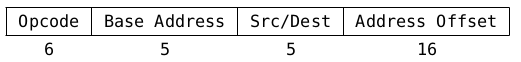
\includegraphics[width=0.7\textwidth]{mips_load_store_instructions}
		\caption{MIPS instruction format for load/store operations}
		\label{fig:mips load store operations}
	\end{figure}
	
	These instructions need to be interpreted differently to register operations and therefore have different opcodes - 35 for \texttt{lw} and 43 for \texttt{sw}. A memory address also has to be specified - which is done in two parts - a \textbf{base} and an \textbf{offset}. The 5 bits allocated to the base address do not specify an address themselves, they specify a register where the address is located. The offset field specifies an address relative to the base.
	
	\subsection{Further MIPS instructions}
		
	
	\section{CPU Microarchitecture}
	The von Neumann model specifies a quite general and non-specific architecture for a computer, but absolutely none of the details. Here we are concerned with the \textbf{microarchitecture}\index{microarchitecture} which refers to the detailed structure and organisation of the machine. This can be divided into two broad parts:
	\begin{itemize}
		\item \textbf{The Datapath}\index{datapath} is a collection of functional units which implement the instruction set. Each functional unit has a specific purpose: the registers are used for storing data, the program counter bookmarks the code; the instruction register stores the current instruction, and the ALU executes arithmetic and logic operations
		
		\item \textbf{The Control Logic}\index{control logic} serves to configure the datapath in the right way so that it implements the desired instruction. It ensures that the correct data is going to the correct functional units, that the results are put in the right place and that the ALU is configured to perform the correct operation on the data. Control is the most complex part of the processor. It's somewhat simple in RISC machines due to the few operations they implement but much harder in CISC machines.
	\end{itemize}
	
	\subsection{MIPS Microarchitecture}
	\subsubsection{Instruction Fetch}
	The first step of the instruction cycle is to get the address of the next instruction and then to fetch that instruction. In order to do this, we need to send the contents of the program counter to memory and bring the contents of that address back to the CPU. We will need to use the \textbf{program counter}, the \textbf{main memory} and the \textbf{instruction register}. The main memory is usually not physically part of the datapath but is integral to its operation, so we will include it in our diagrams.
	
	\par We can put these components together that implements the first stage quite simply. We send the contents of the program counter to the memory via the \textbf{address bus}\index{address bus}. The returned instruction is then loaded into the instruction register via the \textbf{data bus}\index{data bus}.
	
	\begin{figure}[ht]
		\centering
		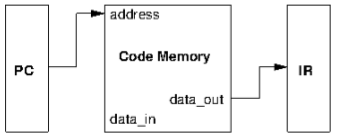
\includegraphics[width=0.4\textwidth]{datapath_instruction_fetch}
		\caption{Datapath elements for instruction fetch}
		\label{fig:datapath instruction fetch}
	\end{figure}
	
	Next, we need to increment the program counter. Commonly this is just adding 4 to the PC to move to the next instruction. In the case of a branch or a jump we may need to make a further adjustment to the PC value, but the constant value of 4 is \textit{always} added. As this is done every cycle we add a simple adder\index{adder} component into the datapath as shown in figure \ref{fig:datapath_pc_adder}.
	
	\begin{figure}[ht]
		\centering
		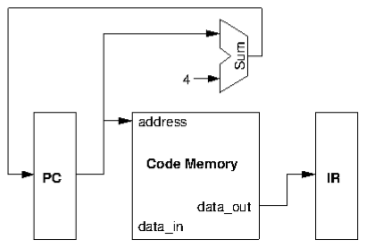
\includegraphics[width=0.5\textwidth]{datapath_pc_adder}
		\caption{We have integrated an adder to increment the PC}
		\label{fig:datapath_pc_adder}
	\end{figure}
	
	\subsubsection{Instruction Execution}
	Whilst we should look at decoding the instruction after fetching it, it's more instructive to look at the datapath components required to actually execute the instruction set after the decoding has been done. Some components required are obvious (such as the ALU and registers), but others are less so.
	
	Registers are required to provide a fast and local amount of memory for a small amount of data items. Any data that is used by an instruction in the MIPS instruction set must be present in the registers as they cannot access external sources (unless they are special load/store instructions). Because of this, we need to provide mechanisms for writing data into the registers and also for reading data from the registers. For some instructions we may need access up to three registers simultaneously. As MIPS has 32 registers, we can use a 5-bit number to uniquely address a single register and these are encoded into the machine code for the instruction. The registers must therefore feature three 5-bit address ports - two of these are for reading and one is for writing - and two 32-bit outputs for retrieving data from the registers. We will also need one final 32-bit input to write data to registers. As not all instructions write to registers we also include an input which signals whether the register specified by the \texttt{write\_addr} is to be written or not. All of these are shown in Figure \ref{fig:registers input output}.
	
	\begin{figure}[ht]
		\centering
		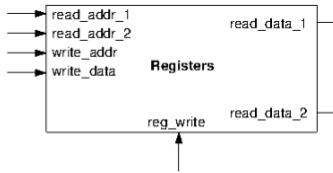
\includegraphics[width=0.6\textwidth]{register_architecture}
		\caption{Registers and their input/output ports}
		\label{fig:registers input output}
	\end{figure}
	
	Next, we would like to build the ALU. The ALU performs all of the processors arithmetic and logic operations and it's internal circuitry must be able to be configured so that it can perform any of the "ALU instructions". In MIPS, the ALU must also be able to compute address, for example, whena address offsets are used - e.g. \texttt{lw \$0, 8(\$sp)}. The ALU handles the addition of the offset. The ALU also handles comparissons required by by branch and set instructions. The ALU must be able to accept up to two 32-bit words from the registers as input, perform the ALU instruction specified in the instruction register as determined by the ALU control unit and to output another 32-bit word (in the case of comparissons, just true/false using the zero output). The ALU is shown in Figure \ref{fig:alu}.
	
	\begin{figure}[ht]
		\centering
		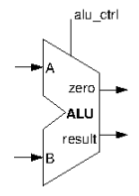
\includegraphics[width=0.2\textwidth]{alu}
		\caption{The ALU and it's input/output ports}
		\label{fig:alu}
	\end{figure}
	
	\par 
	The registers and parts we have shown so far form the basis for a datapath that can execute R-type instructions (e.g. \texttt{add}). Fifteen bits are dedicated to selecting registers that are involved in ALU computations. We can pass these register addresses directly into the register address ports to select the correct registers. The remaining 17 bits are used by the control to configure the datapath to perform the instruction. This gives us the datapath shown in Figure \ref{fig:r type datapath} for these R-type instructions. 

	\begin{figure}[ht]
		\centering
		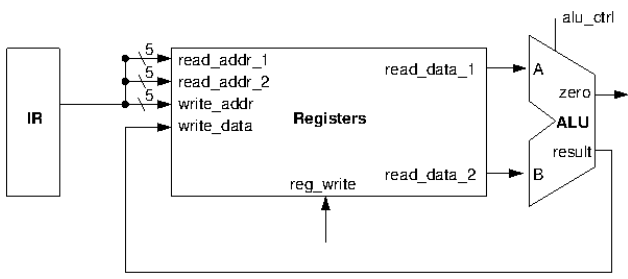
\includegraphics[width = 0.9\textwidth]{r_type_datapath}
		\caption{The datapath for R-type instructions}
		\label{fig:r type datapath}
	\end{figure}
	
	\par 
	Load/store operations are somewhat more complex instructions. They need read and write access to both the registers and main memory, as well as to be able to use the ALU to calculate addresses. A source/destination register address is specified dependent on whether the operation is a load/store. The register of the \textbf{base address} is also specified and the 16-bit address \textbf{offset}. The addition of the base address and the offset is performed by the ALU in the MIPS architecture, but is not as straightforward as it might seem. The base address is 32-bits, whilst the offset is 16-bits. We need to add a new unit to 'extend' the offset so it can be added to the base. This seems trivial (just prepend some zeroes), but branches can go backwards and forwards in the code so we must allow for negative offsets using the two's complement representation. The manipulations that are required to translate the offset are performed by the \textbf{sign extension unit}\index{sign extension unit}. Once the address is computed by adding the offset to the base address, we must read or write the memory address that we have computed, as well as update the contents of the specified register is we are loading. A signal to the memory that controls whether is is a read or write that will be generated by the CPU control unit. We omit this for now to focus on the flow of data.
	
	\begin{figure}[ht]
		\centering
		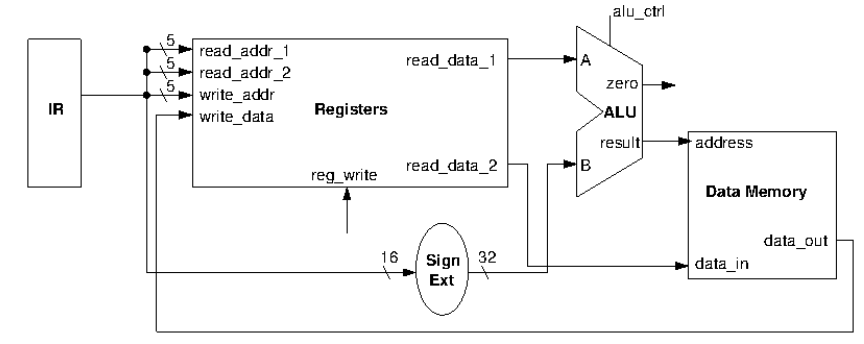
\includegraphics[width=0.9\textwidth]{load_store_instructions_datapath}
		\caption{The datapath for load/store instructions}
		\label{fig:load store instructions datapath}
	\end{figure}
	
	\subsubsection{Branches and Jumps}
	Both branches and jumps achieve essentially the same result - they both have to change the contents of the program counter. The datapath mechanisms are essentially the same because of this, but the control differs depending on the specific instruction being executed as branches require a comparisson to be done. We will deal with branches first, and add jumps later.
	
	\par 
	In order to execute a branch, we have to look at the type of instructions, which is the same as I-type load/store instructions. In the \texttt{beq} instruction for example, we must compare the contents of the two registers specified in the instructions and if they are equal, we add the specified offset to the program counter. Otherwise we increment the PC by 4 as normal. The ALU is capable of performing comparrisons, and the registers are used to store the quanitites to be compared. We will also have to extend the offset to 32-bits from 16-bits in order to add it to the PC. As we need the ALU for the comparisson, we use a dedicated adder instead of the ALU for the bit extension. This incurs a little overhead but reduces overall complexity. The resulting datapath is shown in Figure \ref{fig:branch jump datapath}.
	
	\begin{figure}
		\centering
		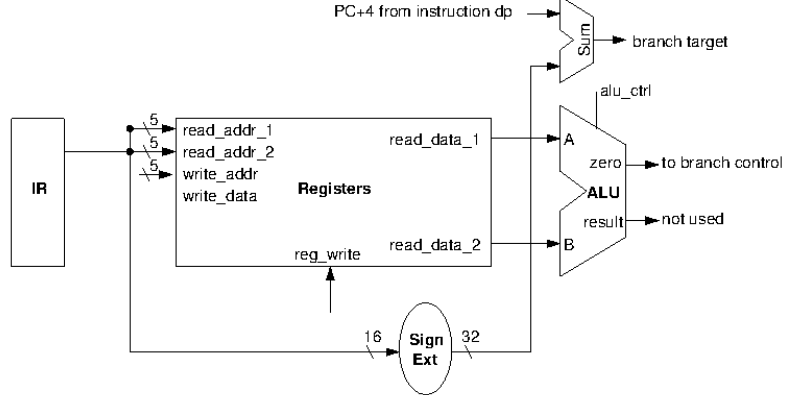
\includegraphics[width=0.9\textwidth]{branch_jump_datapath}
		\caption{Datapath for branch instructions}
		\label{fig:branch jump datapath}
	\end{figure}			
	
	\subsection{Integrating the Datapath}
	We've constructed datapath circuits for a range of the most common MIPS instructions, each of which has their own special requirements. Many of them also have a lot in common, and many of the functional units are used in more than on instruction type. Duplicating functional units is clearly undesirable and because of this we need to be able to control the flow of data within the datapath to ensure that the correct units are employed for each instruction. An example of why this is difficult is that data can be written into the registers from either the ALU or from the data memory, but only one set of wires which these pieces of data can be sent and we cannot simultaneously send two pieces of data down the same wires. The solution is to add switches to the wires, which is known as \textbf{multiplexing}\index{multiplexing}. 
	\par 
	A 2-1 multiplexer is a switch which allows one of the inputs to pass, based on a control signal $C$. With $N$ control wires, we can choose $2^{N}$ inputs. For example, an 8-1 multiplexer will require 3 control wires. Multiplexing will allow us to combine and integrate different sections of the datapath that we designed for the different types of instruction. Firstly, we will integrate the ALU-based instructions which use the IR, the ALU and the registers; and the load-store instructions which use the IR, the registers, the ALU, data memory and a sign extension unit. The challenge is to integrate these two datapaths using only one ALU, and one set of registers. The two datapaths we are trying to integrate can be seen in Figures \ref{fig:r type datapath} and \ref{fig:load store instructions datapath}.
	
	\par 
	In an ALU instruction, the ALU inputs both come from the registers, and the result of the operation is written back to the registers. In a load/store instruction, the ALU inputs are from the registers and sign-extension unit, whilst the registers need to be written by the data memory. Therefore we need to multiplex the data that is to be written into the registers; and the ALU inputs, as show in \ref{fig:alu load store datapath}.
	
	\begin{figure}
		\centering
		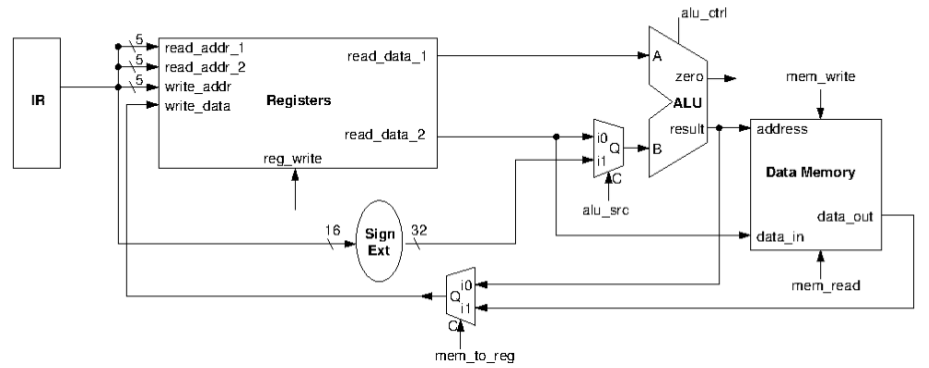
\includegraphics[width=\textwidth]{alu_load_store_datapath}
		\caption{The integrated datapath for ALU and load/store instructions}
		\label{fig:alu load store datapath}
	\end{figure}		
	
	\subsection{CPU Control}
	
	\section{Digital Logic}
	\subsection{Digital Logic}
	\subsubsection{Transistors}
	The basic building block of the modern integrated circuit CPU is the \textbf{transistor}\index{transistor}. For the purpose of this course, we only need to know the transistors are essentially switches which are controlled by their gate voltage. Depending on the type of transistor (NMOS\index{NMOS} or PMOS\index{PMOS}), they will either conduct or not conduct when a voltage is applied to the gate. An NMOS transistor will conduct when the gate is at a positive voltage , and a PMOS transistor will conduct when the gate has no voltage - otherwise it doesn't conduct.
	
	\begin{figure}[h]
	\begin{minipage}[t]{.45\textwidth}
		\caption{(Left) Circuit symbol for an NMOS transistor.  (Right) Circuit symbol for a PMOS transistor}
		\vspace{15pt}
		\centering
		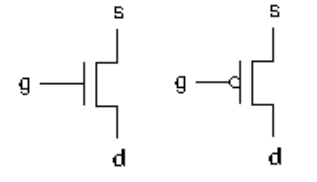
\includegraphics[width=0.45\textwidth]{transistors}
		\label{fig:transistors}
	\end{minipage}
	\hfill
	\begin{minipage}[t]{.45\textwidth}
		\caption{The logical operator \textbf{NOT} built from transistors}
		\vspace{15pt}
		\centering
		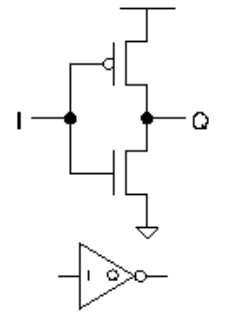
\includegraphics[width=0.45\textwidth]{not_gate_transistors}
		\label{fig:not_transistors}
	\end{minipage}
	\end{figure}
	
	So far data and instructions have been represented by binary digits that have two possible states - zero or one. These states correspond to zero and positive voltages in physical circuits. The zero voltage is usually called \textbf{gnd}\index{gnd}(ground) and the positive voltage \textbf{vdd}\index{vdd}. A signal that has a connection to gnd is in logic state 'zero', and a signal that has a connection to vdd is in logic state 'one'. Using transistors we can transform signals between 'zero' and 'one' states. To begin with, lets implement an inverter circuit which is identical to the logical operation \textbf{not}\index{not gate} as shown in Figure \ref{fig:not_transistors}.	
	
	When the input is at low voltage (zero), the lower NMOS transistor is non-conductive but the top PMOS transistor is conductive. The output therefore becomes connected through the PMOS transistor and is therefore logical 'one'. When the input is at high voltage (one), the PMOS transistor is non-conducting while the NMOS transistor is conducting. Q is therefore connected to gnd via the NMOS transistor and is logical 'zero'. We can see dependent on the input, the output of the circuit will be its inverse and it implements the logical \textbf{NOT} operator.
	
	Similarly, we can implement other basic logical operators from a few transistors. While we might want to make \textbf{AND} and \textbf{OR} straight away, it's actually easier to implement their negated versions - \textbf{NAND} and \textbf{NOR}. We can do both of these in just four transistors, but it requires six to implement their non negated versions.
	
	\begin{figure}[ht]
		\centering
		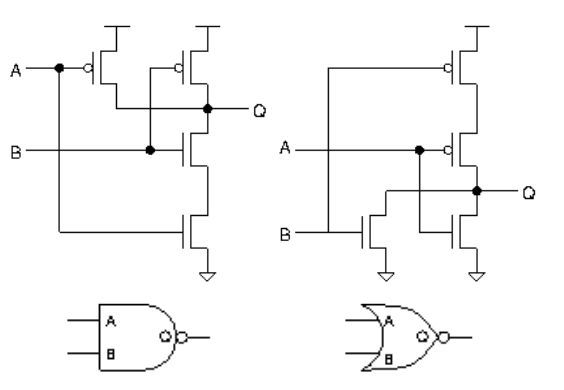
\includegraphics[width=0.6\textwidth]{nand_nor_transistors}
		\caption{(Left) A \textbf{NAND} gate built from four transistors.  (Right) A \textbf{NOR} gate built from four transistors}
		\label{fig:nand_nor_transistors}
	\end{figure}
	
	\subsubsection{Decoders}
	\par 
	\textbf{Combinational logic}\index{combinational logic} is the general term for blocks of digital logic which contain no form of memory - the input must be determined solely by it inputs - and is made from networks of the simple logic gates we have just defined. Example of combinational logic we have seen whilst building the MIPS datapath include multiplexers, simple adders, and even an entire (non-pipelined) ALU.
	
	\par 
	Consider a simple block of combinational logic with two inputs and four outputs - a decoder. This is designed so that each of the four possible input combinations uniquely selects only one of the four outputs. This circuit is common in memories where it is used to select a unique memory location based on the presented address. We start by describing the truth table for this circuit as shown in the figure below. By inspecting the truth table, we can construct its function as a set of logic equations shown next to the truth table.
	\begin{figure}[h]
		\begin{minipage}[t]{.45\textwidth}
			\centering
			\begin{tabular}{c c | c c c c}
				i0 & i1 & Q1 & Q2 & Q3 & Q4  \\ \hline
				0 & 0 & 1 & 0 & 0 & 0 \\
				0 & 1 & 0 & 1 & 0 & 0 \\
				1 & 0 & 0 & 0 & 1 & 0 \\
				1 & 1 & 0 & 0 & 0 & 1
			\end{tabular}
			\caption{Truth table for a two input decoder}
			\label{fig:truth table two input decoder}
		\end{minipage}
		\hfill
		\begin{minipage}[t]{.45\textwidth}
			\begin{itemize}
				\item $Q_{1} = \neg A \wedge \neg B$
				\item $Q_{2} = \neg A \wedge B$
				\item $Q_{3} = A \wedge \neg B$
				\item $Q_{4} = A \wedge B$
			\end{itemize}
		\end{minipage}
	\end{figure}
	
	From here it becomes trivial to translate this into a circuit diagram - you simply have to read off the logical operations (here, the mixtures of \textbf{NOT} and \textbf{AND}) and insert the appropriate gates.
	\begin{figure}[h]
		\centering
		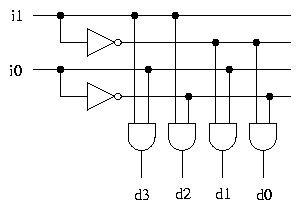
\includegraphics[width=0.5\textwidth]{2_4_decoder}
		\caption{A 2-4 decoder built from logic gates}
		\label{fig:2 4 decoder}
	\end{figure}
	
	\subsubsection{Multiplexers}
	We can also build \textbf{multiplexers}\index{multiplexer} which are a very common component in the CPU. 2-1 Multiplexers are described by the logic equation $Q = (S \wedge I_{1}) \vee (\neg S \wedge I_{0})$, and the truth table is shown below.	Just as we did for a 2-4 decoder, we can easily build a 2-1 multiplexer from a few logic gates as described by its logic equation. In order to build 32-bit multiplexers, all we require are 32 single-bit multiplexers which share the same select signal 'S'.
	
	\begin{figure}[ht]
		\begin{minipage}[t]{0.45\textwidth}
			\centering
			\begin{tabular}{c c | c | c}
				i0 & i1 & S & Q \\ \hline
				0 & 0 & 0 & 0 \\
				0 & 0 & 1 & 0 \\
				0 & 1 & 0 & 0 \\
				0 & 1 & 1 & 1 \\
				1 & 0 & 0 & 1 \\
				1 & 0 & 1 & 0 \\
				1 & 1 & 0 & 1 \\
				1 & 1 & 1 & 1 \\
			\end{tabular}
			\caption{Truth table for a 2-1 multiplexer}
		\label{fig:2 1 multiplexer}
		\end{minipage}
		\hfill
		\begin{minipage}[t]{0.45\textwidth}
			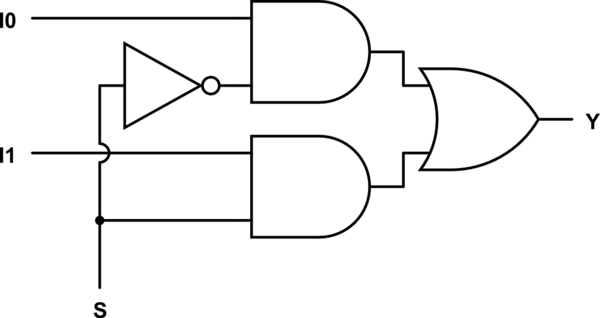
\includegraphics[width=1\textwidth]{2_1_multiplexer}
			\caption{A 2-1 multiplexer built from logic gates}
			\label{fig:2 1 multiplexer}
		\end{minipage}
	\end{figure}
	
	\subsubsection{A Simple Adder}
	An \textbf{adder}\index{adder} is used both in the ALU and in several other places of the datapath. We will design a circuit which is able to add unsigned integers, two's-complement integers and both unsigned and two's-complement fixed-point numbers. For single digit binary addition, we know that $0 + 0 = 0$, $1 + 0 = 0 + 1 = 1$ and $1 + 1 = 0$ with a carry bit of $1$. The carry bit of $1 + 1$ means we will need to introduce a second output which will function as our carry bit. It follows that we can easily express the carry bit as $C = A \wedge B$. In order to do the sum itself we need to introduce a new logical operation, \textbf{exclusive-OR} (otherwise known as \textbf{XOR})\index{exclusive OR}. \textbf{XOR} is indentical to and \textbf{OR} gate but does not output $1$ if both input are also $1$. Using and \textbf{XOR} we can fully implement single-bit addition. The circuit which achieves this is commonly called a \textbf{half-adder}\index{half-adder}.
	
	\begin{figure}[ht]
		\centering
		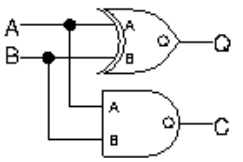
\includegraphics[width=0.3\textwidth]{single_bit_adder}
		\caption{Logic gates which implemet a half-adder}
		\label{fig:half adder}
	\end{figure}
	
	This is clearly very limited as it can only add single bits together and we would like to add multiple-bit binary numbers. We can use a half-adder for the least-significant bit, but for higher bits we need to be able to carry in the the carry bit from the preceeding bit. We can easily achieve the sum using a pair of half-adders where the first adds $I_{1}$ to $I_{2}$, and the second adds the result of the previous to $C_{in}$. The carry bit of this addition is then the \textbf{XOR} of the carry bits from the two half-adders.
	
	\begin{figure}[ht]
		\centering
		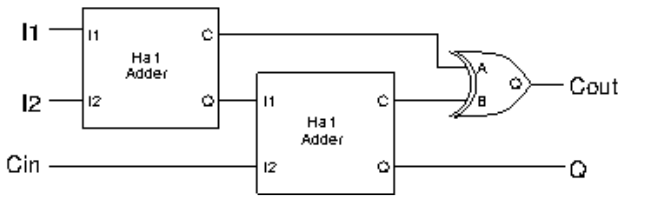
\includegraphics[width=0.8\textwidth]{full_adder}
		\caption{A full-adder built from two half adders and an \textbf{XOR} gate}
		\label{fig:full_adder}
	\end{figure}
	
	We can now join lots of full adders (and one half-adder for the least-significant bit) together to create on single 32-bit adder. The carry bit from the most significant bit in the calculation will be used to indicate \textbf{overflow}\index{overflow} (the result was too large to store in 32-bits).
	
	\subsubsection{A Simple ALU}
	Now we can build an adder, we can put together a simple ALU which can achieve addition of two numbers, bitwise-AND and bitwise-OR. To do this we take our 32-bit adder and modify it by adding one \textbf{AND} gate per bit and one \textbf{OR} bit per bit (with some multiplexers to select the operation we actually want to perform). We can then program the ALU by using the ALUOp signal to select the chosen function. How to build this ALU is shown in Figure \ref{fig:simple ALU}. It is not too dificult to see how you could add additional functionality from here.
	
	\begin{figure}[ht]
		\centering
		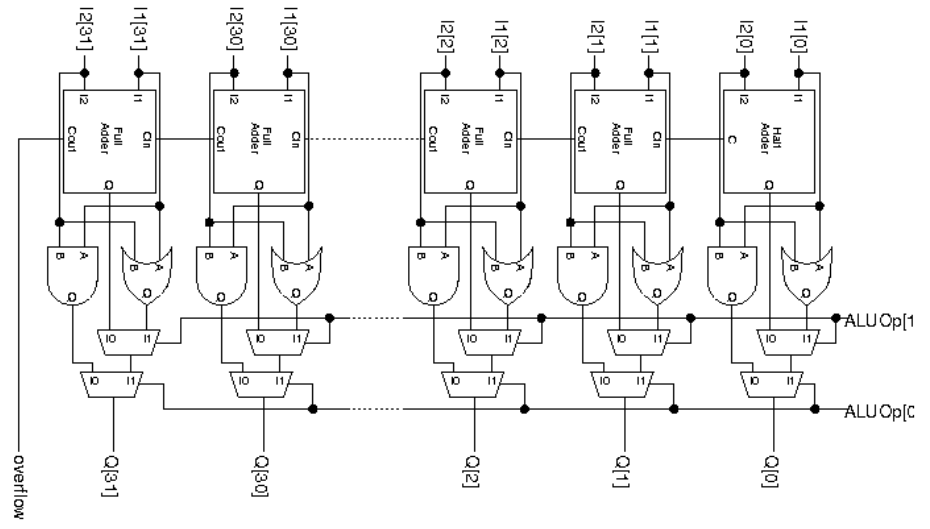
\includegraphics[width=1\textwidth]{simple_ALU}
		\caption{A simple ALU capable of performing addition, bitwise-AND and bitwise-OR operations}
		\label{fig:simple ALU}
	\end{figure}	
	
	\subsection{Number Representation}
	\subsubsection{Positive Integers}
	The simplest of numbers we can represent in a binary computer system are positive (or unsigned) integers. This is the simple binary representation that we have already seen before and are common with. In principle, any natural positive number can be represented, but there are practical limitations. Modern computers break data into 32 or 64-bit chunks (referred to as words), which limits the size of numbers that we can store. With $n$ bits, we can store integers from 0 to $2^{n} - 1$.
	
	\par 
	Long binary strings are tedious for humans to manipulate and mistakes are easily made. It's common to represent numbers in another base for this reason. Commonly, hexadecimal (base-16) is used. We need 16 symbols to represent values. We us the normal 10 decimal symbols, plus A-F. For example, the value of \texttt{0x1C3F} in decimal is:
	\[ (1 \times 16^{3}) + (12 \times 16^{2}) + (3 \times 16^{1}) + (15 \times 16^{0}) = 4096 + 3072 + 48 + 15 = 7231 \]
	
	As 16 is an integer power of 2, converting between binary and hexadecimal is simply a matter of string substitution. Each group of four bits can be converted directly to their hex equivalent and vice-versa.
	
	\subsubsection{Positive Real Numbers}
	We can extend our representation of unsigned integers to unsigned reals (such as $2.1$, $3.14$ etc). We do so by allowing a decimal point in our binary number, and extending the powers backwards from 0. 
	
	\begin{align*}
	101.001_{2} &= (1 \times 2^{2}) + (1 \times 2^{0}) + (1 \times 2^{-3}) \\
				&= 4 + 1 + \frac{1}{8}									   \\
				&= 5\frac{1}{8}                                            \\
	\end{align*}		
	
	We have a choice to make, where do we put the decimal point? Modern computers have 32 or 64-bit words, but many real numbers are still impossible to represent with this. Dependent on the position of the decimal point, we can have an increased accuracy of numbers we can represent or a larger range of values. It's common practice to fix the decimal point at a known location, for example 16-bits for each side. This is called the \textbf{fixed point} representation \index{fixed point representation}.
	
	\subsubsection{Negative Numbers and Two's Complement}
	One possible way to implement negative numbers in binary is to allocate one of the bits as a sign bit. It makes sense to make this the leftmost bit, as the sign of a calculation cannot be determined until the whole calculation has been done. To do this, we either need an extra bit to represent out numbers or to reduce the range of numbers that we can represent. This method is not optimal for the computer. Take the following example: \texttt{01011010} and \texttt{10100110} are the negative of each other as they add to give 0 (ignoring any overflow). They are called each other's \textbf{two's complement}\index{two's complement}. This is a convenient way of representing both positive and negative numbers. To form a numbers two's complement:
	\begin{enumerate}
		\item Invert all bits
		\item Add 1 to the LSB
	\end{enumerate}
	
	If we treat positive numbers to always begin with zero, and be otherwise identical to unsigned numbers then it follows that negative numbers must begin with at least one leading one. We'll consider the sum $(7 - 15)_{10}$ (which is equivalent to $(\texttt{00111} - \texttt{01111})_{2}$) and use two's complement to complete this. We convert $\texttt{01111}_{2}$ to it's two's complement and get $\texttt{10001}_{2}$. Now we can add to get $(\texttt{00111} + \texttt{10001} = \texttt{11000})_{2}$. As the lead digit is 1, this must be a negative number. We take its two's complement by inverting all bits, and adding 1 to get $\texttt{01000}_{2}$. 
	
	\par The range of numbers we can represent in two's complement is different than the number of bits we have. The largest positive value is \texttt{0111...11}, and the smallest positive value is \texttt{000...01}. For negative numbers, the smallest ('least negative') value we can represent is \texttt{111...11} whilst the largest ('most negative') is \texttt{100...00}. Therefore, the range of values that can be represented in two's complement is from $-2^{n-1}$ to $2^{n-1} - 1$
	
	\subsubsection{Floating Point Numbers}
	We can now represent both integers and real numbers (positive and negative) using \textbf{fixed-point} methods. These methods have restrictions. They impose considerable restrictions on the range of numbers that are available to use. Take for example an eight bit representation in two's complement using five bits to store the integer, and three bits to store the non-integer. This is bound by the following limits:
	
	\begin{tabular}{c | c c}
	& Two's Complement & Radix 10 \\ \hline
	Largest Positive Value & \texttt{01111.111} & 15.875 \\
	Smallest Positive Value & \texttt{00000.001} & 0.125 \\
	Largest Negative Value & \texttt{10000.000} & -16 \\
	Smallest Negative Value & \texttt{11111.111} & -0.125
	\end{tabular}
	
	\par 	
	The range of values supported is rather small, and the precision available is also very limited. Fixed point data has a limited range and limited precision. We can circumvent this partially by allocating more bits, but there are practical limitations on this. To support more accurate numerical calculation, a \textbf{floating-point number}\index{floating-point number} type has been devised. Our representation has two parts: the \textbf{mantissa}\index{mantissa} $M$ (sometimes called argument, fraction or significand) and the \textbf{exponent}\index{exponent} $E$ which are combined to give a value $V$ in the following way:
	\[ V = M \times 2^{E} \]
	
	In 8-bits, allowing four bits of mantissa and four of exponent, and placing the radix point after the first bit of the mantissa we have (using two's complement for both exponent and mantissa):
	
	\begin{tabular}{c | c c}
	& Floating Point & Radix 10 \\ \hline
	Largest Positive Value & \texttt{0.111}$\times 2^{\texttt{0111}}$ & $112$ \\
	Smallest Positive Value & \texttt{0.001}$\times 2^{\texttt{1000}}$ & $4.9 \times 10^{-4}$ \\
	Largest Negative Value & \texttt{1.000}$\times 2^{\texttt{0111}}$ & $-128$ \\
	Smallest Negative Value & \texttt{1.111}$\times 2^{\texttt{1000}}$ & $-4.9 \times 10^{-4}$
	\end{tabular}	
	
	As it can be seen, there is a greatly increased range of values available from the exact same amount of bits. This comes at the cost of resolution. The use on an exponent means that the increments are non-linear, and hence larger numbers have a lower resolution than smaller numbers. As a result, you should be extremely careful when using floating point numbers.
	
	Floating-point arithmetic is rather complex and the details are beyond the scope of this module.
	
	\subsection{Clocked Logic}
	
	\section{I/O and Peripherals}
	
	\section{Improving Performance}
	\subsection{Caches and Virtual Memory}
	\subsection{Pipelining and Branch Prediction}
	
	\newpage
	\listoffigures
	\printindex	
\end{document}
